
    




    
\documentclass[11pt]{article}

    
    \usepackage[breakable]{tcolorbox}
    \tcbset{nobeforeafter} % prevents tcolorboxes being placing in paragraphs
    \usepackage{float}
    \floatplacement{figure}{H} % forces figures to be placed at the correct location
    
    \usepackage[T1]{fontenc}
    % Nicer default font (+ math font) than Computer Modern for most use cases
    \usepackage{mathpazo}

    % Basic figure setup, for now with no caption control since it's done
    % automatically by Pandoc (which extracts ![](path) syntax from Markdown).
    \usepackage{graphicx}
    % We will generate all images so they have a width \maxwidth. This means
    % that they will get their normal width if they fit onto the page, but
    % are scaled down if they would overflow the margins.
    \makeatletter
    \def\maxwidth{\ifdim\Gin@nat@width>\linewidth\linewidth
    \else\Gin@nat@width\fi}
    \makeatother
    \let\Oldincludegraphics\includegraphics
    % Set max figure width to be 80% of text width, for now hardcoded.
    \renewcommand{\includegraphics}[1]{\Oldincludegraphics[width=.8\maxwidth]{#1}}
    % Ensure that by default, figures have no caption (until we provide a
    % proper Figure object with a Caption API and a way to capture that
    % in the conversion process - todo).
    \usepackage{caption}
    \DeclareCaptionLabelFormat{nolabel}{}
    \captionsetup{labelformat=nolabel}

    \usepackage{adjustbox} % Used to constrain images to a maximum size 
    \usepackage{xcolor} % Allow colors to be defined
    \usepackage{enumerate} % Needed for markdown enumerations to work
    \usepackage{geometry} % Used to adjust the document margins
    \usepackage{amsmath} % Equations
    \usepackage{amssymb} % Equations
    \usepackage{textcomp} % defines textquotesingle
    % Hack from http://tex.stackexchange.com/a/47451/13684:
    \AtBeginDocument{%
        \def\PYZsq{\textquotesingle}% Upright quotes in Pygmentized code
    }
    \usepackage{upquote} % Upright quotes for verbatim code
    \usepackage{eurosym} % defines \euro
    \usepackage[mathletters]{ucs} % Extended unicode (utf-8) support
    \usepackage[utf8x]{inputenc} % Allow utf-8 characters in the tex document
    \usepackage{fancyvrb} % verbatim replacement that allows latex
    \usepackage{grffile} % extends the file name processing of package graphics 
                         % to support a larger range 
    % The hyperref package gives us a pdf with properly built
    % internal navigation ('pdf bookmarks' for the table of contents,
    % internal cross-reference links, web links for URLs, etc.)
    \usepackage{hyperref}
    \usepackage{longtable} % longtable support required by pandoc >1.10
    \usepackage{booktabs}  % table support for pandoc > 1.12.2
    \usepackage[inline]{enumitem} % IRkernel/repr support (it uses the enumerate* environment)
    \usepackage[normalem]{ulem} % ulem is needed to support strikethroughs (\sout)
                                % normalem makes italics be italics, not underlines
    \usepackage{mathrsfs}
    

    
    % Colors for the hyperref package
    \definecolor{urlcolor}{rgb}{0,.145,.698}
    \definecolor{linkcolor}{rgb}{.71,0.21,0.01}
    \definecolor{citecolor}{rgb}{.12,.54,.11}

    % ANSI colors
    \definecolor{ansi-black}{HTML}{3E424D}
    \definecolor{ansi-black-intense}{HTML}{282C36}
    \definecolor{ansi-red}{HTML}{E75C58}
    \definecolor{ansi-red-intense}{HTML}{B22B31}
    \definecolor{ansi-green}{HTML}{00A250}
    \definecolor{ansi-green-intense}{HTML}{007427}
    \definecolor{ansi-yellow}{HTML}{DDB62B}
    \definecolor{ansi-yellow-intense}{HTML}{B27D12}
    \definecolor{ansi-blue}{HTML}{208FFB}
    \definecolor{ansi-blue-intense}{HTML}{0065CA}
    \definecolor{ansi-magenta}{HTML}{D160C4}
    \definecolor{ansi-magenta-intense}{HTML}{A03196}
    \definecolor{ansi-cyan}{HTML}{60C6C8}
    \definecolor{ansi-cyan-intense}{HTML}{258F8F}
    \definecolor{ansi-white}{HTML}{C5C1B4}
    \definecolor{ansi-white-intense}{HTML}{A1A6B2}
    \definecolor{ansi-default-inverse-fg}{HTML}{FFFFFF}
    \definecolor{ansi-default-inverse-bg}{HTML}{000000}

    % commands and environments needed by pandoc snippets
    % extracted from the output of `pandoc -s`
    \providecommand{\tightlist}{%
      \setlength{\itemsep}{0pt}\setlength{\parskip}{0pt}}
    \DefineVerbatimEnvironment{Highlighting}{Verbatim}{commandchars=\\\{\}}
    % Add ',fontsize=\small' for more characters per line
    \newenvironment{Shaded}{}{}
    \newcommand{\KeywordTok}[1]{\textcolor[rgb]{0.00,0.44,0.13}{\textbf{{#1}}}}
    \newcommand{\DataTypeTok}[1]{\textcolor[rgb]{0.56,0.13,0.00}{{#1}}}
    \newcommand{\DecValTok}[1]{\textcolor[rgb]{0.25,0.63,0.44}{{#1}}}
    \newcommand{\BaseNTok}[1]{\textcolor[rgb]{0.25,0.63,0.44}{{#1}}}
    \newcommand{\FloatTok}[1]{\textcolor[rgb]{0.25,0.63,0.44}{{#1}}}
    \newcommand{\CharTok}[1]{\textcolor[rgb]{0.25,0.44,0.63}{{#1}}}
    \newcommand{\StringTok}[1]{\textcolor[rgb]{0.25,0.44,0.63}{{#1}}}
    \newcommand{\CommentTok}[1]{\textcolor[rgb]{0.38,0.63,0.69}{\textit{{#1}}}}
    \newcommand{\OtherTok}[1]{\textcolor[rgb]{0.00,0.44,0.13}{{#1}}}
    \newcommand{\AlertTok}[1]{\textcolor[rgb]{1.00,0.00,0.00}{\textbf{{#1}}}}
    \newcommand{\FunctionTok}[1]{\textcolor[rgb]{0.02,0.16,0.49}{{#1}}}
    \newcommand{\RegionMarkerTok}[1]{{#1}}
    \newcommand{\ErrorTok}[1]{\textcolor[rgb]{1.00,0.00,0.00}{\textbf{{#1}}}}
    \newcommand{\NormalTok}[1]{{#1}}
    
    % Additional commands for more recent versions of Pandoc
    \newcommand{\ConstantTok}[1]{\textcolor[rgb]{0.53,0.00,0.00}{{#1}}}
    \newcommand{\SpecialCharTok}[1]{\textcolor[rgb]{0.25,0.44,0.63}{{#1}}}
    \newcommand{\VerbatimStringTok}[1]{\textcolor[rgb]{0.25,0.44,0.63}{{#1}}}
    \newcommand{\SpecialStringTok}[1]{\textcolor[rgb]{0.73,0.40,0.53}{{#1}}}
    \newcommand{\ImportTok}[1]{{#1}}
    \newcommand{\DocumentationTok}[1]{\textcolor[rgb]{0.73,0.13,0.13}{\textit{{#1}}}}
    \newcommand{\AnnotationTok}[1]{\textcolor[rgb]{0.38,0.63,0.69}{\textbf{\textit{{#1}}}}}
    \newcommand{\CommentVarTok}[1]{\textcolor[rgb]{0.38,0.63,0.69}{\textbf{\textit{{#1}}}}}
    \newcommand{\VariableTok}[1]{\textcolor[rgb]{0.10,0.09,0.49}{{#1}}}
    \newcommand{\ControlFlowTok}[1]{\textcolor[rgb]{0.00,0.44,0.13}{\textbf{{#1}}}}
    \newcommand{\OperatorTok}[1]{\textcolor[rgb]{0.40,0.40,0.40}{{#1}}}
    \newcommand{\BuiltInTok}[1]{{#1}}
    \newcommand{\ExtensionTok}[1]{{#1}}
    \newcommand{\PreprocessorTok}[1]{\textcolor[rgb]{0.74,0.48,0.00}{{#1}}}
    \newcommand{\AttributeTok}[1]{\textcolor[rgb]{0.49,0.56,0.16}{{#1}}}
    \newcommand{\InformationTok}[1]{\textcolor[rgb]{0.38,0.63,0.69}{\textbf{\textit{{#1}}}}}
    \newcommand{\WarningTok}[1]{\textcolor[rgb]{0.38,0.63,0.69}{\textbf{\textit{{#1}}}}}
    
    
    % Define a nice break command that doesn't care if a line doesn't already
    % exist.
    \def\br{\hspace*{\fill} \\* }
    % Math Jax compatibility definitions
    \def\gt{>}
    \def\lt{<}
    \let\Oldtex\TeX
    \let\Oldlatex\LaTeX
    \renewcommand{\TeX}{\textrm{\Oldtex}}
    \renewcommand{\LaTeX}{\textrm{\Oldlatex}}
    % Document parameters
    % Document title
    \title{Final-Copy1}
    
    
    
    
    
% Pygments definitions
\makeatletter
\def\PY@reset{\let\PY@it=\relax \let\PY@bf=\relax%
    \let\PY@ul=\relax \let\PY@tc=\relax%
    \let\PY@bc=\relax \let\PY@ff=\relax}
\def\PY@tok#1{\csname PY@tok@#1\endcsname}
\def\PY@toks#1+{\ifx\relax#1\empty\else%
    \PY@tok{#1}\expandafter\PY@toks\fi}
\def\PY@do#1{\PY@bc{\PY@tc{\PY@ul{%
    \PY@it{\PY@bf{\PY@ff{#1}}}}}}}
\def\PY#1#2{\PY@reset\PY@toks#1+\relax+\PY@do{#2}}

\expandafter\def\csname PY@tok@w\endcsname{\def\PY@tc##1{\textcolor[rgb]{0.73,0.73,0.73}{##1}}}
\expandafter\def\csname PY@tok@c\endcsname{\let\PY@it=\textit\def\PY@tc##1{\textcolor[rgb]{0.25,0.50,0.50}{##1}}}
\expandafter\def\csname PY@tok@cp\endcsname{\def\PY@tc##1{\textcolor[rgb]{0.74,0.48,0.00}{##1}}}
\expandafter\def\csname PY@tok@k\endcsname{\let\PY@bf=\textbf\def\PY@tc##1{\textcolor[rgb]{0.00,0.50,0.00}{##1}}}
\expandafter\def\csname PY@tok@kp\endcsname{\def\PY@tc##1{\textcolor[rgb]{0.00,0.50,0.00}{##1}}}
\expandafter\def\csname PY@tok@kt\endcsname{\def\PY@tc##1{\textcolor[rgb]{0.69,0.00,0.25}{##1}}}
\expandafter\def\csname PY@tok@o\endcsname{\def\PY@tc##1{\textcolor[rgb]{0.40,0.40,0.40}{##1}}}
\expandafter\def\csname PY@tok@ow\endcsname{\let\PY@bf=\textbf\def\PY@tc##1{\textcolor[rgb]{0.67,0.13,1.00}{##1}}}
\expandafter\def\csname PY@tok@nb\endcsname{\def\PY@tc##1{\textcolor[rgb]{0.00,0.50,0.00}{##1}}}
\expandafter\def\csname PY@tok@nf\endcsname{\def\PY@tc##1{\textcolor[rgb]{0.00,0.00,1.00}{##1}}}
\expandafter\def\csname PY@tok@nc\endcsname{\let\PY@bf=\textbf\def\PY@tc##1{\textcolor[rgb]{0.00,0.00,1.00}{##1}}}
\expandafter\def\csname PY@tok@nn\endcsname{\let\PY@bf=\textbf\def\PY@tc##1{\textcolor[rgb]{0.00,0.00,1.00}{##1}}}
\expandafter\def\csname PY@tok@ne\endcsname{\let\PY@bf=\textbf\def\PY@tc##1{\textcolor[rgb]{0.82,0.25,0.23}{##1}}}
\expandafter\def\csname PY@tok@nv\endcsname{\def\PY@tc##1{\textcolor[rgb]{0.10,0.09,0.49}{##1}}}
\expandafter\def\csname PY@tok@no\endcsname{\def\PY@tc##1{\textcolor[rgb]{0.53,0.00,0.00}{##1}}}
\expandafter\def\csname PY@tok@nl\endcsname{\def\PY@tc##1{\textcolor[rgb]{0.63,0.63,0.00}{##1}}}
\expandafter\def\csname PY@tok@ni\endcsname{\let\PY@bf=\textbf\def\PY@tc##1{\textcolor[rgb]{0.60,0.60,0.60}{##1}}}
\expandafter\def\csname PY@tok@na\endcsname{\def\PY@tc##1{\textcolor[rgb]{0.49,0.56,0.16}{##1}}}
\expandafter\def\csname PY@tok@nt\endcsname{\let\PY@bf=\textbf\def\PY@tc##1{\textcolor[rgb]{0.00,0.50,0.00}{##1}}}
\expandafter\def\csname PY@tok@nd\endcsname{\def\PY@tc##1{\textcolor[rgb]{0.67,0.13,1.00}{##1}}}
\expandafter\def\csname PY@tok@s\endcsname{\def\PY@tc##1{\textcolor[rgb]{0.73,0.13,0.13}{##1}}}
\expandafter\def\csname PY@tok@sd\endcsname{\let\PY@it=\textit\def\PY@tc##1{\textcolor[rgb]{0.73,0.13,0.13}{##1}}}
\expandafter\def\csname PY@tok@si\endcsname{\let\PY@bf=\textbf\def\PY@tc##1{\textcolor[rgb]{0.73,0.40,0.53}{##1}}}
\expandafter\def\csname PY@tok@se\endcsname{\let\PY@bf=\textbf\def\PY@tc##1{\textcolor[rgb]{0.73,0.40,0.13}{##1}}}
\expandafter\def\csname PY@tok@sr\endcsname{\def\PY@tc##1{\textcolor[rgb]{0.73,0.40,0.53}{##1}}}
\expandafter\def\csname PY@tok@ss\endcsname{\def\PY@tc##1{\textcolor[rgb]{0.10,0.09,0.49}{##1}}}
\expandafter\def\csname PY@tok@sx\endcsname{\def\PY@tc##1{\textcolor[rgb]{0.00,0.50,0.00}{##1}}}
\expandafter\def\csname PY@tok@m\endcsname{\def\PY@tc##1{\textcolor[rgb]{0.40,0.40,0.40}{##1}}}
\expandafter\def\csname PY@tok@gh\endcsname{\let\PY@bf=\textbf\def\PY@tc##1{\textcolor[rgb]{0.00,0.00,0.50}{##1}}}
\expandafter\def\csname PY@tok@gu\endcsname{\let\PY@bf=\textbf\def\PY@tc##1{\textcolor[rgb]{0.50,0.00,0.50}{##1}}}
\expandafter\def\csname PY@tok@gd\endcsname{\def\PY@tc##1{\textcolor[rgb]{0.63,0.00,0.00}{##1}}}
\expandafter\def\csname PY@tok@gi\endcsname{\def\PY@tc##1{\textcolor[rgb]{0.00,0.63,0.00}{##1}}}
\expandafter\def\csname PY@tok@gr\endcsname{\def\PY@tc##1{\textcolor[rgb]{1.00,0.00,0.00}{##1}}}
\expandafter\def\csname PY@tok@ge\endcsname{\let\PY@it=\textit}
\expandafter\def\csname PY@tok@gs\endcsname{\let\PY@bf=\textbf}
\expandafter\def\csname PY@tok@gp\endcsname{\let\PY@bf=\textbf\def\PY@tc##1{\textcolor[rgb]{0.00,0.00,0.50}{##1}}}
\expandafter\def\csname PY@tok@go\endcsname{\def\PY@tc##1{\textcolor[rgb]{0.53,0.53,0.53}{##1}}}
\expandafter\def\csname PY@tok@gt\endcsname{\def\PY@tc##1{\textcolor[rgb]{0.00,0.27,0.87}{##1}}}
\expandafter\def\csname PY@tok@err\endcsname{\def\PY@bc##1{\setlength{\fboxsep}{0pt}\fcolorbox[rgb]{1.00,0.00,0.00}{1,1,1}{\strut ##1}}}
\expandafter\def\csname PY@tok@kc\endcsname{\let\PY@bf=\textbf\def\PY@tc##1{\textcolor[rgb]{0.00,0.50,0.00}{##1}}}
\expandafter\def\csname PY@tok@kd\endcsname{\let\PY@bf=\textbf\def\PY@tc##1{\textcolor[rgb]{0.00,0.50,0.00}{##1}}}
\expandafter\def\csname PY@tok@kn\endcsname{\let\PY@bf=\textbf\def\PY@tc##1{\textcolor[rgb]{0.00,0.50,0.00}{##1}}}
\expandafter\def\csname PY@tok@kr\endcsname{\let\PY@bf=\textbf\def\PY@tc##1{\textcolor[rgb]{0.00,0.50,0.00}{##1}}}
\expandafter\def\csname PY@tok@bp\endcsname{\def\PY@tc##1{\textcolor[rgb]{0.00,0.50,0.00}{##1}}}
\expandafter\def\csname PY@tok@fm\endcsname{\def\PY@tc##1{\textcolor[rgb]{0.00,0.00,1.00}{##1}}}
\expandafter\def\csname PY@tok@vc\endcsname{\def\PY@tc##1{\textcolor[rgb]{0.10,0.09,0.49}{##1}}}
\expandafter\def\csname PY@tok@vg\endcsname{\def\PY@tc##1{\textcolor[rgb]{0.10,0.09,0.49}{##1}}}
\expandafter\def\csname PY@tok@vi\endcsname{\def\PY@tc##1{\textcolor[rgb]{0.10,0.09,0.49}{##1}}}
\expandafter\def\csname PY@tok@vm\endcsname{\def\PY@tc##1{\textcolor[rgb]{0.10,0.09,0.49}{##1}}}
\expandafter\def\csname PY@tok@sa\endcsname{\def\PY@tc##1{\textcolor[rgb]{0.73,0.13,0.13}{##1}}}
\expandafter\def\csname PY@tok@sb\endcsname{\def\PY@tc##1{\textcolor[rgb]{0.73,0.13,0.13}{##1}}}
\expandafter\def\csname PY@tok@sc\endcsname{\def\PY@tc##1{\textcolor[rgb]{0.73,0.13,0.13}{##1}}}
\expandafter\def\csname PY@tok@dl\endcsname{\def\PY@tc##1{\textcolor[rgb]{0.73,0.13,0.13}{##1}}}
\expandafter\def\csname PY@tok@s2\endcsname{\def\PY@tc##1{\textcolor[rgb]{0.73,0.13,0.13}{##1}}}
\expandafter\def\csname PY@tok@sh\endcsname{\def\PY@tc##1{\textcolor[rgb]{0.73,0.13,0.13}{##1}}}
\expandafter\def\csname PY@tok@s1\endcsname{\def\PY@tc##1{\textcolor[rgb]{0.73,0.13,0.13}{##1}}}
\expandafter\def\csname PY@tok@mb\endcsname{\def\PY@tc##1{\textcolor[rgb]{0.40,0.40,0.40}{##1}}}
\expandafter\def\csname PY@tok@mf\endcsname{\def\PY@tc##1{\textcolor[rgb]{0.40,0.40,0.40}{##1}}}
\expandafter\def\csname PY@tok@mh\endcsname{\def\PY@tc##1{\textcolor[rgb]{0.40,0.40,0.40}{##1}}}
\expandafter\def\csname PY@tok@mi\endcsname{\def\PY@tc##1{\textcolor[rgb]{0.40,0.40,0.40}{##1}}}
\expandafter\def\csname PY@tok@il\endcsname{\def\PY@tc##1{\textcolor[rgb]{0.40,0.40,0.40}{##1}}}
\expandafter\def\csname PY@tok@mo\endcsname{\def\PY@tc##1{\textcolor[rgb]{0.40,0.40,0.40}{##1}}}
\expandafter\def\csname PY@tok@ch\endcsname{\let\PY@it=\textit\def\PY@tc##1{\textcolor[rgb]{0.25,0.50,0.50}{##1}}}
\expandafter\def\csname PY@tok@cm\endcsname{\let\PY@it=\textit\def\PY@tc##1{\textcolor[rgb]{0.25,0.50,0.50}{##1}}}
\expandafter\def\csname PY@tok@cpf\endcsname{\let\PY@it=\textit\def\PY@tc##1{\textcolor[rgb]{0.25,0.50,0.50}{##1}}}
\expandafter\def\csname PY@tok@c1\endcsname{\let\PY@it=\textit\def\PY@tc##1{\textcolor[rgb]{0.25,0.50,0.50}{##1}}}
\expandafter\def\csname PY@tok@cs\endcsname{\let\PY@it=\textit\def\PY@tc##1{\textcolor[rgb]{0.25,0.50,0.50}{##1}}}

\def\PYZbs{\char`\\}
\def\PYZus{\char`\_}
\def\PYZob{\char`\{}
\def\PYZcb{\char`\}}
\def\PYZca{\char`\^}
\def\PYZam{\char`\&}
\def\PYZlt{\char`\<}
\def\PYZgt{\char`\>}
\def\PYZsh{\char`\#}
\def\PYZpc{\char`\%}
\def\PYZdl{\char`\$}
\def\PYZhy{\char`\-}
\def\PYZsq{\char`\'}
\def\PYZdq{\char`\"}
\def\PYZti{\char`\~}
% for compatibility with earlier versions
\def\PYZat{@}
\def\PYZlb{[}
\def\PYZrb{]}
\makeatother


    % For linebreaks inside Verbatim environment from package fancyvrb. 
    \makeatletter
        \newbox\Wrappedcontinuationbox 
        \newbox\Wrappedvisiblespacebox 
        \newcommand*\Wrappedvisiblespace {\textcolor{red}{\textvisiblespace}} 
        \newcommand*\Wrappedcontinuationsymbol {\textcolor{red}{\llap{\tiny$\m@th\hookrightarrow$}}} 
        \newcommand*\Wrappedcontinuationindent {3ex } 
        \newcommand*\Wrappedafterbreak {\kern\Wrappedcontinuationindent\copy\Wrappedcontinuationbox} 
        % Take advantage of the already applied Pygments mark-up to insert 
        % potential linebreaks for TeX processing. 
        %        {, <, #, %, $, ' and ": go to next line. 
        %        _, }, ^, &, >, - and ~: stay at end of broken line. 
        % Use of \textquotesingle for straight quote. 
        \newcommand*\Wrappedbreaksatspecials {% 
            \def\PYGZus{\discretionary{\char`\_}{\Wrappedafterbreak}{\char`\_}}% 
            \def\PYGZob{\discretionary{}{\Wrappedafterbreak\char`\{}{\char`\{}}% 
            \def\PYGZcb{\discretionary{\char`\}}{\Wrappedafterbreak}{\char`\}}}% 
            \def\PYGZca{\discretionary{\char`\^}{\Wrappedafterbreak}{\char`\^}}% 
            \def\PYGZam{\discretionary{\char`\&}{\Wrappedafterbreak}{\char`\&}}% 
            \def\PYGZlt{\discretionary{}{\Wrappedafterbreak\char`\<}{\char`\<}}% 
            \def\PYGZgt{\discretionary{\char`\>}{\Wrappedafterbreak}{\char`\>}}% 
            \def\PYGZsh{\discretionary{}{\Wrappedafterbreak\char`\#}{\char`\#}}% 
            \def\PYGZpc{\discretionary{}{\Wrappedafterbreak\char`\%}{\char`\%}}% 
            \def\PYGZdl{\discretionary{}{\Wrappedafterbreak\char`\$}{\char`\$}}% 
            \def\PYGZhy{\discretionary{\char`\-}{\Wrappedafterbreak}{\char`\-}}% 
            \def\PYGZsq{\discretionary{}{\Wrappedafterbreak\textquotesingle}{\textquotesingle}}% 
            \def\PYGZdq{\discretionary{}{\Wrappedafterbreak\char`\"}{\char`\"}}% 
            \def\PYGZti{\discretionary{\char`\~}{\Wrappedafterbreak}{\char`\~}}% 
        } 
        % Some characters . , ; ? ! / are not pygmentized. 
        % This macro makes them "active" and they will insert potential linebreaks 
        \newcommand*\Wrappedbreaksatpunct {% 
            \lccode`\~`\.\lowercase{\def~}{\discretionary{\hbox{\char`\.}}{\Wrappedafterbreak}{\hbox{\char`\.}}}% 
            \lccode`\~`\,\lowercase{\def~}{\discretionary{\hbox{\char`\,}}{\Wrappedafterbreak}{\hbox{\char`\,}}}% 
            \lccode`\~`\;\lowercase{\def~}{\discretionary{\hbox{\char`\;}}{\Wrappedafterbreak}{\hbox{\char`\;}}}% 
            \lccode`\~`\:\lowercase{\def~}{\discretionary{\hbox{\char`\:}}{\Wrappedafterbreak}{\hbox{\char`\:}}}% 
            \lccode`\~`\?\lowercase{\def~}{\discretionary{\hbox{\char`\?}}{\Wrappedafterbreak}{\hbox{\char`\?}}}% 
            \lccode`\~`\!\lowercase{\def~}{\discretionary{\hbox{\char`\!}}{\Wrappedafterbreak}{\hbox{\char`\!}}}% 
            \lccode`\~`\/\lowercase{\def~}{\discretionary{\hbox{\char`\/}}{\Wrappedafterbreak}{\hbox{\char`\/}}}% 
            \catcode`\.\active
            \catcode`\,\active 
            \catcode`\;\active
            \catcode`\:\active
            \catcode`\?\active
            \catcode`\!\active
            \catcode`\/\active 
            \lccode`\~`\~ 	
        }
    \makeatother

    \let\OriginalVerbatim=\Verbatim
    \makeatletter
    \renewcommand{\Verbatim}[1][1]{%
        %\parskip\z@skip
        \sbox\Wrappedcontinuationbox {\Wrappedcontinuationsymbol}%
        \sbox\Wrappedvisiblespacebox {\FV@SetupFont\Wrappedvisiblespace}%
        \def\FancyVerbFormatLine ##1{\hsize\linewidth
            \vtop{\raggedright\hyphenpenalty\z@\exhyphenpenalty\z@
                \doublehyphendemerits\z@\finalhyphendemerits\z@
                \strut ##1\strut}%
        }%
        % If the linebreak is at a space, the latter will be displayed as visible
        % space at end of first line, and a continuation symbol starts next line.
        % Stretch/shrink are however usually zero for typewriter font.
        \def\FV@Space {%
            \nobreak\hskip\z@ plus\fontdimen3\font minus\fontdimen4\font
            \discretionary{\copy\Wrappedvisiblespacebox}{\Wrappedafterbreak}
            {\kern\fontdimen2\font}%
        }%
        
        % Allow breaks at special characters using \PYG... macros.
        \Wrappedbreaksatspecials
        % Breaks at punctuation characters . , ; ? ! and / need catcode=\active 	
        \OriginalVerbatim[#1,codes*=\Wrappedbreaksatpunct]%
    }
    \makeatother

    % Exact colors from NB
    \definecolor{incolor}{HTML}{303F9F}
    \definecolor{outcolor}{HTML}{D84315}
    \definecolor{cellborder}{HTML}{CFCFCF}
    \definecolor{cellbackground}{HTML}{F7F7F7}
    
    % prompt
    \newcommand{\prompt}[4]{
        \llap{{\color{#2}[#3]: #4}}\vspace{-1.25em}
    }
    

    
    % Prevent overflowing lines due to hard-to-break entities
    \sloppy 
    % Setup hyperref package
    \hypersetup{
      breaklinks=true,  % so long urls are correctly broken across lines
      colorlinks=true,
      urlcolor=urlcolor,
      linkcolor=linkcolor,
      citecolor=citecolor,
      }
    % Slightly bigger margins than the latex defaults
    
    \geometry{verbose,tmargin=1in,bmargin=1in,lmargin=1in,rmargin=1in}
    
    

    \begin{document}
    
    
    \maketitle
    
    

    
    \begin{tcolorbox}[breakable, size=fbox, boxrule=1pt, pad at break*=1mm,colback=cellbackground, colframe=cellborder]
\prompt{In}{incolor}{1}{\hspace{4pt}}
\begin{Verbatim}[commandchars=\\\{\}]
\PY{k+kn}{from} \PY{n+nn}{IPython} \PY{k}{import} \PY{n}{get\PYZus{}ipython}\PY{p}{;}   
\PY{n}{get\PYZus{}ipython}\PY{p}{(}\PY{p}{)}\PY{o}{.}\PY{n}{magic}\PY{p}{(}\PY{l+s+s1}{\PYZsq{}}\PY{l+s+s1}{reset \PYZhy{}sf}\PY{l+s+s1}{\PYZsq{}}\PY{p}{)}
\PY{c+c1}{\PYZsh{}https://github.com/kirbs\PYZhy{}/hide\PYZus{}code}
\end{Verbatim}
\end{tcolorbox}

    \begin{tcolorbox}[breakable, size=fbox, boxrule=1pt, pad at break*=1mm,colback=cellbackground, colframe=cellborder]
\prompt{In}{incolor}{2}{\hspace{4pt}}
\begin{Verbatim}[commandchars=\\\{\}]
\PY{o}{\PYZpc{}}\PY{k}{run} \PYZhy{}i Packages.py
\PY{o}{\PYZpc{}}\PY{k}{matplotlib} inline
\PY{o}{\PYZpc{}}\PY{k}{load\PYZus{}ext} rpy2.ipython
\end{Verbatim}
\end{tcolorbox}

    \begin{tcolorbox}[breakable, size=fbox, boxrule=1pt, pad at break*=1mm,colback=cellbackground, colframe=cellborder]
\prompt{In}{incolor}{3}{\hspace{4pt}}
\begin{Verbatim}[commandchars=\\\{\}]
\PY{o}{\PYZpc{}\PYZpc{}}\PY{k}{R}
library(ggplot2)
library(readr)
library(lubridate)
library(dplyr)
library(tidyr)
library(viridis)
\end{Verbatim}
\end{tcolorbox}

    \hypertarget{abstract}{%
\section{Abstract}\label{abstract}}

    

    \hypertarget{background}{%
\section{Background}\label{background}}

    \hypertarget{introduction}{%
\subsection{Introduction}\label{introduction}}

    \hypertarget{the-world-wide-web-and-economic-prosperity}{%
\subsubsection{The World Wide Web and Economic
Prosperity}\label{the-world-wide-web-and-economic-prosperity}}

    Since the inception of the first home computers in 1977
(REF)\cite{7169703/23A77C9T}, modern society has become utterly
dependent on and indeed, inexorably bound to digital technology. The
rapid and widespread adoption of computational technology has led to the
fastest rate of societal and economic development our species has ever
experienced. One need only consider that between the years of X and Y,
\#\#\#\# number of people gained access to the WWW {[}mention benefits
of WWW for end users?{]}, to appreciate the magnitude of this digital
technology. Such rapid and widespread adoption has created a seemingly
insatiable demand for \_\_.

\begin{figure}
  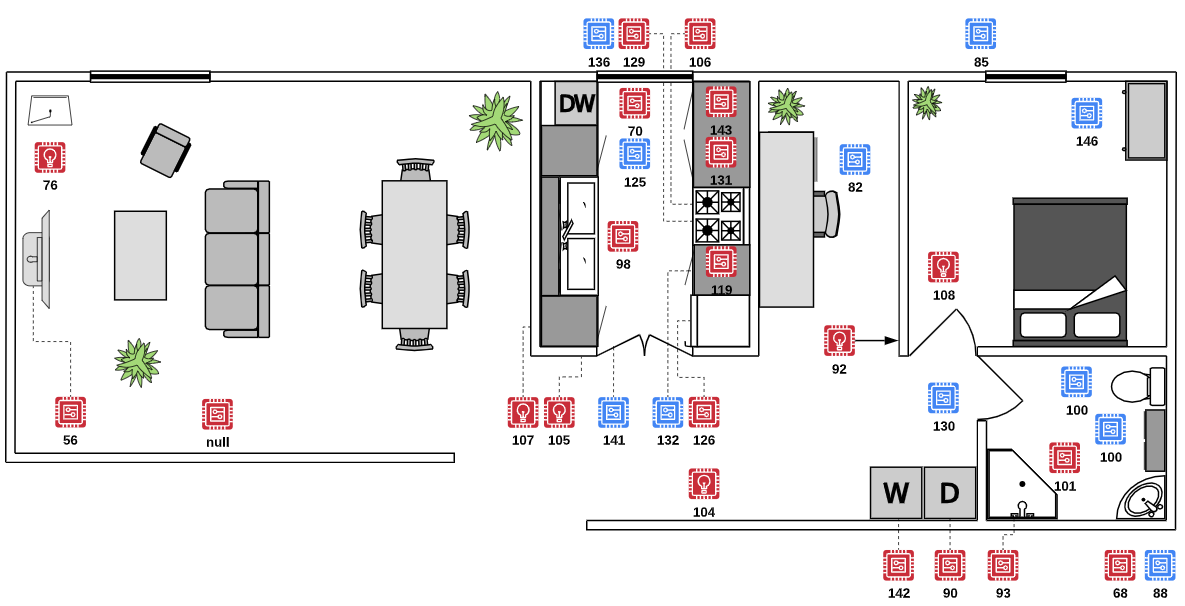
\includegraphics[width=\linewidth]{boat.jpg}
  \caption{A boat.}
  \label{fig:boat1}
\end{figure}

Figure \ref{fig:boat1} shows a boat.

Indeed, our quest for exponentially greater computational power and
digital storage capacity has led to a new and utterly ubiquitous
technological paradigm; Cloud Computing (REF), defined as; The practice
of using a network of remote servers hosted on the Internet to store,
manage, and process data, rather than a local server or a personal
computer (https://www.dictionary.com/browse/cloud-computing).

As with the original WWW, Cloud Computing itself acts as a facilitator
for new technologies. One such example being the Internet of Things
(IoT) paradigm. The Internet of Things can be surmised as the extension
of the Internet and the Web into the physical realm, by means of the
widespread deployment of spatially distributed devices with embedded
identification, sensing and/or actuation capabilities
{[}@article\{miorandi2012\}{]}. The Internet of Things (IoT) paradigm
enables physical devices to connect and exchange information, and also
allows objects to be sensed or controlled remotely through the internet
(@article\{huang2018\} @ 1 of @article\{huang2018\}) The IoT paradigm
enables physical devices to connect and exchange information. IoT
devices allow objects to be sensed or controlled remotely through the
Internet {[}@article\{atzori2010\}{]}. IoT thus represents a convergence
of real-world objects and digital objects into seamless (seamless?) and
unified cyber-physical system.

Considering again the bigger picture of societal benefit, Figure X,
shows that the benefits of technological deployment have been widely
adopted and exploited. However, the success of modern human society is
not without consequence. Paradoxically, all of the benefits our society
has enjoyed from the development, production and deployment of
technology, has required vast amounts of energy. This energy has, since
the industrial revolution, primarily been derived from the burning of
fossil fuels (REF). The International Panel on Climate Change (IPCC)
estimates that ABC by XYZ if we do not do blah (REF). As exemplified by
figure Y (co-inciding to the time period of figure X) global greenhouse
gas emissions are steadily increasing (REF). At the current rate, blah
et al estimate that in 20\#\#, humans will be living in an atmospheric
conditions not experienced since \#\#\#\# the mezozoic era, XX years
before the evolution of modern humans (REF, REF).

It is therefore imperative moving forward as a species that all steps
are be taken to mitigate the emission of greenhouse gases and abate the
advance of anthropomorphic climate change. The scale of the challenge is
such that technology itself will prove critical in effectively
combatting this extential threat to civilisation. When considering
energy consumption, the industrial sector (including the non-combusted
use of fuels) currently consumes around half of all global energy and
feedstock fuels, with residential and commercial buildings (29\%) and
transport (21\%) accounting for the remainder
(https://www.bp.com/en/global/corporate/energy-economics/energy-outlook/demand-by-sector.html).

With residential and commercial buildings accounting for 29\% of energy
demand globally (REF). A qualitative assessment of figures X Y and Z
show that our increased energy consumption has coincided with our
staggerings global acheivements, including lifting millions out of
poverty blah blah blah. We have more development we use more energy, but
we have more development we are better off in all ways. We ALSO have
more internet connectivity.

It therefore stands that the key to continues human prosperity is to
de-couple energy demand growth from economic growth. Clearly economic
prosperity is a direct contributing factor to human prosperity in
general. One such avenue for reduced energy consumption is the
optimization of existing services, utilities, and so on.

residential and commercial energy consumption

The convergence of

explosive growth of our population

https://ourworldindata.org/energy-production-and-changing-energy-sources
https://www.iea.org/statistics/kwes/consumption/

    

    \hypertarget{datasets}{%
\subsection{Datasets}\label{datasets}}

    \hypertarget{data-preprocessing-and-visualisation}{%
\section{Data Preprocessing and
Visualisation}\label{data-preprocessing-and-visualisation}}

    \hypertarget{importing-preprocessing-the-activities-meta-data}{%
\subsection{Importing \& Preprocessing the Activities Meta
Data}\label{importing-preprocessing-the-activities-meta-data}}

    The dataset \texttt{S1Activities.csv} was imported into the Jupyter
interactive environment. These data contains a tabulated summary of
Heading, Category, Subcategory and a corresponding code. After
importation, the dataset has dimensionality of {[}3, 33{]}, with
\texttt{Heading}, \texttt{Category} \& \texttt{Subcategory} present as
non-null objects. The attribute \texttt{Code} (which codefies the unique
set of Heading, Category) was imported as an index value. At this time,
the activities data will not be subject to preprocessing.

    \begin{tcolorbox}[breakable, size=fbox, boxrule=1pt, pad at break*=1mm,colback=cellbackground, colframe=cellborder]
\prompt{In}{incolor}{22}{\hspace{4pt}}
\begin{Verbatim}[commandchars=\\\{\}]
\PY{n}{ds} \PY{o}{=} \PY{n}{pd}\PY{o}{.}\PY{n}{read\PYZus{}csv}\PY{p}{(}\PY{n}{PATH} \PY{o}{+} \PY{l+s+s1}{\PYZsq{}}\PY{l+s+s1}{/datasets/S1Activities.csv}\PY{l+s+s1}{\PYZsq{}}\PY{p}{,} \PY{n}{index\PYZus{}col} \PY{o}{=} \PY{l+s+s1}{\PYZsq{}}\PY{l+s+s1}{Code}\PY{l+s+s1}{\PYZsq{}}\PY{p}{)} 
\PY{n}{ds}\PY{o}{.}\PY{n}{head}\PY{p}{(}\PY{n}{n}\PY{o}{=}\PY{l+m+mi}{5}\PY{p}{)}  
\end{Verbatim}
\end{tcolorbox}

            \begin{tcolorbox}[breakable, boxrule=.5pt, size=fbox, pad at break*=1mm, opacityfill=0]
\prompt{Out}{outcolor}{22}{\hspace{3.5pt}}
\begin{Verbatim}[commandchars=\\\{\}]
                 Heading                 Category        Subcategory
Code
1     Employment related  Employment work at home       Work at home
5     Employment related        Travel employment  Going out to work
10        Personal needs                   Eating             Eating
15        Personal needs         Personal hygiene          Toileting
20        Personal needs         Personal hygiene            Bathing
\end{Verbatim}
\end{tcolorbox}
        
    \hypertarget{importing-preprocessing-the-sensor-meta-data}{%
\subsection{Importing \& Preprocessing the Sensor Meta
Data}\label{importing-preprocessing-the-sensor-meta-data}}

    The dataset \texttt{S1sensors.csv} was imported into the Jupyter
interactive environment. These data contains a tabulated values for
Sensor ID, Room and Sensor Activity Type, with no header row present in
the original dataset. After importation, the dataset has dimensionality
of {[}3, 76{]}, with header \texttt{0}, \texttt{1} \& \texttt{2}
corresponding to \texttt{SensorID}, \texttt{Room} \&
\texttt{Sensor\ Activity\ Type}, respectively. All attributes are
nominal, and were imported as dtype str, accordingly. Note that it can
be immediately seen (\texttt{dsS1Sensors.head()}) that attribute
\texttt{1} \& \texttt{2} contain degenerate values. This will be
addressed in the subsequent data preprocessing.

The preprocessing of the sensor data is a critical step in our analysis.
Careful consideration of the data, including the presence of duplicates.
This is because if we dont have a sufficient understanding of where and
why duplicates exist, we will not be able to satisfactorarily preprocess
them. Failure to do so we mean that there is potentail degeneracy in our
source dataset, leading to unknown issues with our downstream analysis.

    \begin{tcolorbox}[breakable, size=fbox, boxrule=1pt, pad at break*=1mm,colback=cellbackground, colframe=cellborder]
\prompt{In}{incolor}{23}{\hspace{4pt}}
\begin{Verbatim}[commandchars=\\\{\}]
\PY{c+c1}{\PYZsh{} Importing the dataset}
\PY{n}{dsS1Sensors} \PY{o}{=} \PY{n}{pd}\PY{o}{.}\PY{n}{read\PYZus{}csv}\PY{p}{(}\PY{n}{PATH} \PY{o}{+} \PY{l+s+s1}{\PYZsq{}}\PY{l+s+s1}{/datasets/S1sensors.csv}\PY{l+s+s1}{\PYZsq{}}\PY{p}{,} 
                          \PY{n}{dtype}\PY{o}{=}\PY{p}{\PYZob{}}\PY{l+m+mi}{0}\PY{p}{:}\PY{n+nb}{str}\PY{p}{,} \PY{l+m+mi}{1}\PY{p}{:}\PY{n+nb}{str}\PY{p}{,} \PY{l+m+mi}{2}\PY{p}{:}\PY{n+nb}{str}\PY{p}{\PYZcb{}}\PY{p}{,}
                          \PY{n}{index\PYZus{}col} \PY{o}{=} \PY{k+kc}{None}\PY{p}{,} \PY{n}{header} \PY{o}{=} \PY{k+kc}{None}\PY{p}{)}
\PY{n}{dsS1Sensors}\PY{o}{.}\PY{n}{head}\PY{p}{(}\PY{p}{)}
\end{Verbatim}
\end{tcolorbox}

            \begin{tcolorbox}[breakable, boxrule=.5pt, size=fbox, pad at break*=1mm, opacityfill=0]
\prompt{Out}{outcolor}{23}{\hspace{3.5pt}}
\begin{Verbatim}[commandchars=\\\{\}]
     0         1              2
0  100  Bathroom  Toilet Flush
1  101  Bathroom   Light switch
2  104     Foyer   Light switch
3  105   Kitchen   Light switch
4  106   Kitchen         Burner
\end{Verbatim}
\end{tcolorbox}
        
    Column {[}1{]} \& Column {[}2{]} of the sensor data will be
concatenated, whitespace will be removed, all text will be cast to
lowercase and a final whitespace strip will be performed. The python
script \texttt{S1sensorsPreprocessing.py} is run perform several
preprocessing steps in these data. The script concatenates the
attributes \texttt{dsS1Sensors{[}1{]}} and \texttt{dsS1Sensors{[}2{]}},
with an underscore. Whitespace is then stripped and all string values
are coerced to lowercase. This newly created attribute is then added to
the dataframe, as seen below (REF). Additionally, the attributes
\texttt{0}, \texttt{1} \& \texttt{2} are renamed \texttt{subActNum},
\texttt{room} \& \texttt{activity}, respectively. - Data types - IF a
sub-act requires electricity

    \begin{tcolorbox}[breakable, size=fbox, boxrule=1pt, pad at break*=1mm,colback=cellbackground, colframe=cellborder]
\prompt{In}{incolor}{24}{\hspace{4pt}}
\begin{Verbatim}[commandchars=\\\{\}]
\PY{o}{\PYZpc{}}\PY{k}{run} \PYZhy{}i S1sensorsPreprocessing.py
\end{Verbatim}
\end{tcolorbox}

    \begin{tcolorbox}[breakable, size=fbox, boxrule=1pt, pad at break*=1mm,colback=cellbackground, colframe=cellborder]
\prompt{In}{incolor}{25}{\hspace{4pt}}
\begin{Verbatim}[commandchars=\\\{\}]
\PY{n}{dsS1Sensors}\PY{o}{.}\PY{n}{head}\PY{p}{(}\PY{p}{)}
\end{Verbatim}
\end{tcolorbox}

            \begin{tcolorbox}[breakable, boxrule=.5pt, size=fbox, pad at break*=1mm, opacityfill=0]
\prompt{Out}{outcolor}{25}{\hspace{3.5pt}}
\begin{Verbatim}[commandchars=\\\{\}]
  subActNum      room       activity                concat
0       100  Bathroom  Toilet Flush   bathroom\_toiletflush
1       101  Bathroom   Light switch  bathroom\_lightswitch
2       104     Foyer   Light switch     foyer\_lightswitch
3       105   Kitchen   Light switch   kitchen\_lightswitch
4       106   Kitchen         Burner        kitchen\_burner
\end{Verbatim}
\end{tcolorbox}
        
    The function \texttt{getUniqueValues.py} is invoked to provide a means
of capturing a list of unique values in a given column of a dataset. The
newly created \texttt{dsS1Sensors} is then checked for duplicates in two
attributes, \texttt{subActNum} \& \texttt{concat}. The number of unique
values in \texttt{dsS1Sensors.subActNum} is found to be 76,
demonstrating that this attribute contains a set of completely unique
values (recall n(rows) = 76). The number of unique values in
\texttt{dsS1Sensors.concat} is found to be 41, demonstrating that
despite the concatenation methodology, their are still duplicate values
in the dataframe. These duplicate values warrant further investigation.
The function \texttt{seen\_dupes\_dsS1Sensors.py} is used to list counts
with their corresponding values.

    \begin{tcolorbox}[breakable, size=fbox, boxrule=1pt, pad at break*=1mm,colback=cellbackground, colframe=cellborder]
\prompt{In}{incolor}{8}{\hspace{4pt}}
\begin{Verbatim}[commandchars=\\\{\}]
\PY{o}{\PYZpc{}}\PY{k}{run} \PYZhy{}i getUniqueValues.py
\end{Verbatim}
\end{tcolorbox}

    \begin{tcolorbox}[breakable, size=fbox, boxrule=1pt, pad at break*=1mm,colback=cellbackground, colframe=cellborder]
\prompt{In}{incolor}{9}{\hspace{4pt}}
\begin{Verbatim}[commandchars=\\\{\}]
\PY{n}{uniqueS1SubActNum} \PY{o}{=} \PY{n}{getUniqueValues}\PY{p}{(}\PY{n}{dsS1Sensors}\PY{o}{.}\PY{n}{iloc}\PY{p}{[}\PY{p}{:}\PY{p}{,}\PY{l+m+mi}{0}\PY{p}{]}\PY{p}{)}
\PY{n+nb}{len}\PY{p}{(}\PY{n}{uniqueS1SubActNum}\PY{p}{)}
\end{Verbatim}
\end{tcolorbox}

            \begin{tcolorbox}[breakable, boxrule=.5pt, size=fbox, pad at break*=1mm, opacityfill=0]
\prompt{Out}{outcolor}{9}{\hspace{3.5pt}}
\begin{Verbatim}[commandchars=\\\{\}]
76
\end{Verbatim}
\end{tcolorbox}
        
    \begin{tcolorbox}[breakable, size=fbox, boxrule=1pt, pad at break*=1mm,colback=cellbackground, colframe=cellborder]
\prompt{In}{incolor}{10}{\hspace{4pt}}
\begin{Verbatim}[commandchars=\\\{\}]
\PY{n}{uniqueS1Sensors} \PY{o}{=} \PY{n}{getUniqueValues}\PY{p}{(}\PY{n}{dsS1Sensors}\PY{o}{.}\PY{n}{iloc}\PY{p}{[}\PY{p}{:}\PY{p}{,}\PY{l+m+mi}{3}\PY{p}{]}\PY{p}{)}
\PY{n+nb}{len}\PY{p}{(}\PY{n}{uniqueS1Sensors}\PY{p}{)}
\end{Verbatim}
\end{tcolorbox}

            \begin{tcolorbox}[breakable, boxrule=.5pt, size=fbox, pad at break*=1mm, opacityfill=0]
\prompt{Out}{outcolor}{10}{\hspace{3.5pt}}
\begin{Verbatim}[commandchars=\\\{\}]
41
\end{Verbatim}
\end{tcolorbox}
        
    \begin{tcolorbox}[breakable, size=fbox, boxrule=1pt, pad at break*=1mm,colback=cellbackground, colframe=cellborder]
\prompt{In}{incolor}{11}{\hspace{4pt}}
\begin{Verbatim}[commandchars=\\\{\}]
\PY{o}{\PYZpc{}}\PY{k}{run} \PYZhy{}i seen\PYZus{}dupes\PYZus{}dsS1Sensors.py
\end{Verbatim}
\end{tcolorbox}

    \begin{Verbatim}[commandchars=\\\{\}]
3   kitchen\_lightswitch
4   kitchen\_burner
2   livingroom\_lightswitch
7   kitchen\_drawer
3   kitchen\_refrigerator
15  kitchen\_cabinet
2   kitchen\_door
5   bedroom\_drawer
2   bathroom\_medicinecabinet
2   bathroom\_cabinet
\end{Verbatim}

    Upon compilation of the above summary list, and with reference to the
original work is was determined that these values result from multiple
sensors with extremely similar functionality. For example,
kitchen\_burner has a value of n=4 - this is because on the burner in
the apartment under investigation, there were 4 individual burners
present. Similarly, kitchen\_cabinet has a value of n=15, indicating
that for the various cabinets in the apartment, each were given sensors.
On the one-hand, this level of granularity may provide fertile grounds
for advanced analysis, HOWEVER, for the purposes of this research
project, such values will serve to increase the dimensionality of the
overall dataset. High dimensionality can lead to difficulties with
plotting, \ldots. ML (REF) and thus IN A SUBSEQUENT PREPROCESSING
exercise these values will be collapsed down to have n=1.

\textbf{Creation of JSON Catalogues PRIOR to dup removal} - why? Because
even if a key-value pair cannot be matched it will simply be ignored
\textbf{Prior to dupe removal} As this work is largely concerned with
energy usage in the home, the sub-activities will be categorized based
on their energy requirement. That is, if a sub-activity requires an
input of energy beyond what the end user alone can provide, it will be
classified as \texttt{energyReq} = true. Whereas, if a sub-activity is
able to be performed through only interaction with the end user, it will
be classified as \texttt{energyReq} = false. By way of example, the
sub-activity \texttt{bathroom\_toiletflush} will have an
\texttt{energyReq} equal to false, while the sub-activity
\texttt{bathroom\_lightswitch} will have an \texttt{energyReq} equal to
true. Each row (n=76) needs to be inspected manually to determine if the
activity requires electricity.

Function \texttt{reqEnergy\_containSpecialChar.py} is run - After visual
inspection, uses
\texttt{reqEnergy\ =\ \textquotesingle{}ligh\textbar{}burn\textbar{}mach\textbar{}toas\textbar{}freez\textbar{}dvd\textbar{}lamp\textbar{}washer\textbar{}dry\textbar{}exh\textbar{}disp\textbar{}frig\textbar{}oven\textbar{}hot\textbar{}micro\textquotesingle{}}
to find subActivities which require energy input beyond that of the end
user - Checked below for SPECIAL CHAR - Special CHARs removed

    \begin{tcolorbox}[breakable, size=fbox, boxrule=1pt, pad at break*=1mm,colback=cellbackground, colframe=cellborder]
\prompt{In}{incolor}{12}{\hspace{4pt}}
\begin{Verbatim}[commandchars=\\\{\}]
\PY{o}{\PYZpc{}}\PY{k}{run} \PYZhy{}i reqEnergy\PYZus{}containSpecialChar.py
\end{Verbatim}
\end{tcolorbox}

    \begin{tcolorbox}[breakable, size=fbox, boxrule=1pt, pad at break*=1mm,colback=cellbackground, colframe=cellborder]
\prompt{In}{incolor}{13}{\hspace{4pt}}
\begin{Verbatim}[commandchars=\\\{\}]
\PY{n}{dsS1Sensors}\PY{o}{.}\PY{n}{loc}\PY{p}{[}\PY{n}{dsS1Sensors}\PY{p}{[}\PY{l+s+s1}{\PYZsq{}}\PY{l+s+s1}{specialChar}\PY{l+s+s1}{\PYZsq{}}\PY{p}{]} \PY{o}{==} \PY{k+kc}{True}\PY{p}{]}                           \PY{c+c1}{\PYZsh{} Filter for true}
\end{Verbatim}
\end{tcolorbox}

            \begin{tcolorbox}[breakable, boxrule=.5pt, size=fbox, pad at break*=1mm, opacityfill=0]
\prompt{Out}{outcolor}{13}{\hspace{3.5pt}}
\begin{Verbatim}[commandchars=\\\{\}]
   subActNum          room      activity                    concat  reqEnergy  \textbackslash{}
58        82  Office/study        Drawer       office/study\_drawer      False
68        92  Office/study  Light switch  office/study\_lightswitch       True

    specialChar
58         True
68         True
\end{Verbatim}
\end{tcolorbox}
        
    \hypertarget{importing-preprocessing-the-activities-data}{%
\subsection{Importing \& Preprocessing the Activities
Data}\label{importing-preprocessing-the-activities-data}}

    The activities data set \texttt{S1activities.csv} will be imported,
evaluated and cleaned. The goal of the pre-processing will be to
restructure the dataset into a `tidy' format, that is, where the
attributes are columns, the rows are instances, and each cell contains
only one value. Given that the data is time-series, timestamps will be
used as indexes. The data will also be cast into continuous 24 hour
segments, with timestamps in the form \texttt{YYYY-MM-DD\ hh:mm:ss}
(using datetime data type)

MENTION THIS FROM Huang et al.~

We aim to perform the preprocessing in such a way that is * minimally
computationally intensive * reproducible / traceable code * reasonable
checks (validation)

Example of ds when opened in Microsoft excel.

The activities data was imported into an indexed dataframe, containing
only one column, with 1475 rows, with all values comma-separated (per
row). This style of import had to be used, due to the varying number of
comma-separated elements in each row (as seen in figure X, above).

\begin{itemize}
\tightlist
\item
  A array of strings, instead of an array of arrays Analysis of the
  original dataset, and exploration during pre-processing to this point,
  shows us that the original dataset follows a structure such that each
  5 rows of data contains is one discrete set of data. In this
  structure,
\item
  Row 1 = Activity, Date, Start Time, End Time
\item
  Row 2 = Sub-activity (an action that can be executed as part of
  performing the activity) code-values
\item
  Row 3 = Sub-activity descriptive values
\item
  Row 4 = Sub-activity start time
\item
  Row 5 = Sub-activity end time In order to access the values
  programmatically, we will now turn the 1D array list back into a 2D
  array list, where each element array{[}i{]} contains the 5 rows of
  information, as described above.
\end{itemize}

The activities data set \texttt{S1activities.csv} will be imported,
evaluated and cleaned. The goal of the pre-processing will be to
restructure the dataset into a `tidy' format, that is, where the
attributes are columns, the rows are instances, and each cell contains
only one value. Given that the data is time-series, timestamps will be
used as indexes. The data will also be cast into continuous 24 hour
segments, with timestamps in the form \texttt{YYYY-MM-DD\ hh:mm:ss}
(using datetime data type)

We aim to perform the preprocessing in such a way that is * minimally
computationally intensive * reproducible / traceable code * reasonable
checks (validation) The activities data was imported into an indexed
dataframe, containing only one column, with 1475 rows, with all values
comma-separated (per row). This style of import had to be used, due to
the varying number of comma-separated elements in each row (as seen in
figure X, above). * A array of strings, instead of an array of arrays
Analysis of the original dataset, and exploration during pre-processing
to this point, shows us that the original dataset follows a structure
such that each 5 rows of data contains is one discrete set of data. In
this structure, * Row 1 = Activity, Date, Start Time, End Time * Row 2 =
Sub-activity (an action that can be executed as part of performing the
activity) code-values * Row 3 = Sub-activity descriptive values * Row 4
= Sub-activity start time * Row 5 = Sub-activity end time In order to
access the values programmatically, we will now turn the 1D array list
back into a 2D array list, where each element array{[}i{]} contains the
5 rows of information, as described above.

    \begin{tcolorbox}[breakable, size=fbox, boxrule=1pt, pad at break*=1mm,colback=cellbackground, colframe=cellborder]
\prompt{In}{incolor}{23}{\hspace{4pt}}
\begin{Verbatim}[commandchars=\\\{\}]
\PY{n}{dsIntermediate}\PY{o}{.}\PY{n}{head}\PY{p}{(}\PY{p}{)}
\end{Verbatim}
\end{tcolorbox}

            \begin{tcolorbox}[breakable, boxrule=.5pt, size=fbox, pad at break*=1mm, opacityfill=0]
\prompt{Out}{outcolor}{23}{\hspace{3.5pt}}
\begin{Verbatim}[commandchars=\\\{\}]
            activity      date startTime   endTime
0            Bathing  4/1/2003  20:41:35  21:32:50
1          Toileting  4/1/2003  17:30:36  17:46:41
2          Toileting  4/1/2003   18:4:43   18:18:2
3          Toileting  4/1/2003   11:52:1  11:58:50
4  Going out to work  4/1/2003  12:11:26  12:15:12
\end{Verbatim}
\end{tcolorbox}
        
    \textbf{Extracting the Activity, Time and Data} If we run
\texttt{a{[}0{]}{[}0{]}}, we get
\texttt{\textquotesingle{}Bathing,4/1/2003,20:41:35,21:32:50\textquotesingle{}}
* A string with 4 comma-separated `items' * We won't check the entire
DF, rather, will rely on errors thrown back to confirm validity
(`validation of the method')

\textbf{Constructing the while loop} * Create empty lists * Extracts the
relevant elements * Adds (appends) the elements to the lists

\textbf{Sanity Checks} * We won't check the entire DF, rather, will rely
on errors thrown back to confirm validity (`validation of the method') *
Divisible by 5

    \begin{tcolorbox}[breakable, size=fbox, boxrule=1pt, pad at break*=1mm,colback=cellbackground, colframe=cellborder]
\prompt{In}{incolor}{24}{\hspace{4pt}}
\begin{Verbatim}[commandchars=\\\{\}]
\PY{n}{ds}\PY{o}{.}\PY{n}{head}\PY{p}{(}\PY{p}{)}
\end{Verbatim}
\end{tcolorbox}

            \begin{tcolorbox}[breakable, boxrule=.5pt, size=fbox, pad at break*=1mm, opacityfill=0]
\prompt{Out}{outcolor}{24}{\hspace{3.5pt}}
\begin{Verbatim}[commandchars=\\\{\}]
            activity               start                 end
0            Bathing 2003-04-01 20:41:35 2003-04-01 21:32:50
1          Toileting 2003-04-01 17:30:36 2003-04-01 17:46:41
2          Toileting 2003-04-01 18:04:43 2003-04-01 18:18:02
3          Toileting 2003-04-01 11:52:01 2003-04-01 11:58:50
4  Going out to work 2003-04-01 12:11:26 2003-04-01 12:15:12
\end{Verbatim}
\end{tcolorbox}
        
    \hypertarget{aggregated-box-plot}{%
\paragraph{Aggregated Box Plot}\label{aggregated-box-plot}}

    \begin{tcolorbox}[breakable, size=fbox, boxrule=1pt, pad at break*=1mm,colback=cellbackground, colframe=cellborder]
\prompt{In}{incolor}{38}{\hspace{4pt}}
\begin{Verbatim}[commandchars=\\\{\}]
\PY{o}{\PYZpc{}\PYZpc{}}\PY{k}{R}
p \PYZlt{}\PYZhy{} ggplot(ds, aes(subAct, durationSec))
p \PYZlt{}\PYZhy{} p + geom\PYZus{}boxplot(fill= \PYZdq{}plum\PYZdq{}, outlier.alpha = 0.8) \PYZsh{} aes(colour = WDWE) \PYZsh{}, outlier.size = 1
p \PYZlt{}\PYZhy{} p + theme(legend.position = \PYZdq{}right\PYZdq{}) + coord\PYZus{}flip() +
  labs(title = \PYZdq{}Box Plots\PYZdq{},
       subtitle = \PYZdq{}Subactivity Duraiton\PYZdq{},
       caption = \PYZdq{}Source: TBU\PYZdq{},
       x = \PYZdq{}SubActivity\PYZdq{},
       y = \PYZdq{}Duration (sec)\PYZdq{})
ggsave(\PYZdq{}images/boxPlots.png\PYZdq{}, plot = last\PYZus{}plot(), device = png(), 
       scale = 1.5, width = 18, height = 16, units = c(\PYZdq{}cm\PYZdq{}), dpi = 300)
\end{Verbatim}
\end{tcolorbox}

    MENTION THIS FROM Huang et al.~ 

    \hypertarget{strip-plots}{%
\paragraph{Strip Plots}\label{strip-plots}}

    Text

    MENTION THIS FROM Huang et al.~

\begin{center}\rule{0.5\linewidth}{\linethickness}\end{center}

    \hypertarget{bathroom-exhaust-fan}{%
\subparagraph{Bathroom Exhaust Fan}\label{bathroom-exhaust-fan}}

    Text

    MENTION THIS FROM Huang et al.~

\begin{center}\rule{0.5\linewidth}{\linethickness}\end{center}

    \hypertarget{kitchen-garbage-disposal}{%
\subparagraph{Kitchen Garbage Disposal}\label{kitchen-garbage-disposal}}

    Text

    MENTION THIS FROM Huang et al.~

\begin{center}\rule{0.5\linewidth}{\linethickness}\end{center}

    \hypertarget{bathroom-toiletflush}{%
\subparagraph{Bathroom Toiletflush}\label{bathroom-toiletflush}}

    Text - ADD LINE SEGMENT CHART

    \hypertarget{sankey-diagrams---qualitative-assessment}{%
\subsection{Sankey Diagrams - Qualitative
Assessment}\label{sankey-diagrams---qualitative-assessment}}

    \begin{tcolorbox}[breakable, size=fbox, boxrule=1pt, pad at break*=1mm,colback=cellbackground, colframe=cellborder]
\prompt{In}{incolor}{68}{\hspace{4pt}}
\begin{Verbatim}[commandchars=\\\{\}]
\PY{k+kn}{from} \PY{n+nn}{IPython}\PY{n+nn}{.}\PY{n+nn}{display} \PY{k}{import} \PY{n}{IFrame}
\PY{n}{IFrame}\PY{p}{(}\PY{n}{src}\PY{o}{=}\PY{l+s+s1}{\PYZsq{}}\PY{l+s+s1}{WeekdayAfternoonds\PYZus{}1n\PYZus{}60s.html}\PY{l+s+s1}{\PYZsq{}}\PY{p}{,} \PY{n}{width}\PY{o}{=}\PY{l+m+mi}{1000}\PY{p}{,} \PY{n}{height}\PY{o}{=}\PY{l+m+mi}{600}\PY{p}{)}
\end{Verbatim}
\end{tcolorbox}

            \begin{tcolorbox}[breakable, boxrule=.5pt, size=fbox, pad at break*=1mm, opacityfill=0]
\prompt{Out}{outcolor}{68}{\hspace{3.5pt}}
\begin{Verbatim}[commandchars=\\\{\}]
<IPython.lib.display.IFrame at 0x12a26e210>
\end{Verbatim}
\end{tcolorbox}
        
    \begin{tcolorbox}[breakable, size=fbox, boxrule=1pt, pad at break*=1mm,colback=cellbackground, colframe=cellborder]
\prompt{In}{incolor}{69}{\hspace{4pt}}
\begin{Verbatim}[commandchars=\\\{\}]
\PY{k+kn}{from} \PY{n+nn}{IPython}\PY{n+nn}{.}\PY{n+nn}{display} \PY{k}{import} \PY{n}{IFrame}
\PY{n}{IFrame}\PY{p}{(}\PY{n}{src}\PY{o}{=}\PY{l+s+s1}{\PYZsq{}}\PY{l+s+s1}{WeekdayAfternoonds\PYZus{}10n\PYZus{}60s.html}\PY{l+s+s1}{\PYZsq{}}\PY{p}{,} \PY{n}{width}\PY{o}{=}\PY{l+m+mi}{1000}\PY{p}{,} \PY{n}{height}\PY{o}{=}\PY{l+m+mi}{600}\PY{p}{)}
\end{Verbatim}
\end{tcolorbox}

            \begin{tcolorbox}[breakable, boxrule=.5pt, size=fbox, pad at break*=1mm, opacityfill=0]
\prompt{Out}{outcolor}{69}{\hspace{3.5pt}}
\begin{Verbatim}[commandchars=\\\{\}]
<IPython.lib.display.IFrame at 0x12a11b3d0>
\end{Verbatim}
\end{tcolorbox}
        

    % Add a bibliography block to the postdoc
    \bibliographystyle{apalike}
    \bibliography{DM}
    
    
    \end{document}
